\documentclass[
  twoside,
  openright,
  degree    = master,               		% degree   = master  | doctor
  language  = chinese,              		% language = chinese | english
  fontset   = template,             		% fontset  = default | template | system | overleaf
]{ccuthesis}

% !TeX root = ./main.tex

% --------------------------------------------------
% 資訊設定(Information Configs)
% --------------------------------------------------

\ccusetup{
  university*   = {National Chung Cheng University},
  university    = {國立中正大學},
  college       = {工學院},
  college*      = {College of Engineering},
  institute     = {電機工程研究所},
  institute*    = {Department of Electrical Engineering}, % 請確認您的科系為Department of xxx或Institute of xxx
  title         = {國立中正大學碩博士畢業論文模版},
  title*        = {National Chung Cheng University (CCU) \\ Thesis/Dissertation Template in \LaTeX},
  author        = {鄭庭安},
  author*       = {Ting-An Cheng},
  advisor       = {余松年},
  advisor*      = {Sung-Nien Yu},
  date          = {一百一十三年~七月},                      % ~ 表示空格
  date*         = {July~2024},
  keywords      = {LaTeX, 中文, 論文, 模板},
  keywords*     = {LaTeX, CJK, Thesis, Template},
}

% --------------------------------------------------
% 加載套件(Include Packages)
% --------------------------------------------------

\usepackage{amsmath, amsthm, amssymb}   % 數學環境
\usepackage{bm}                         % 數學符號加粗
\usepackage{ulem}                       % 下劃線、雙下劃線與波浪紋效果
\usepackage{booktabs}                   % 改善表格設置
\usepackage{multirow}                   % 合併儲存格
\usepackage{diagbox}                    % 插入表格反斜線
\usepackage{array}                      % 調整表格高度
\usepackage{longtable}                  % 支援跨頁長表格
\usepackage{threeparttable}             % 表格加註解
\usepackage{paralist, enumitem}         % 列表環境
\usepackage{zhnumber}                   % 中文數字
\usepackage{algorithm, algpseudocode}   % 演算法
\usepackage{graphics, graphicx}         % 圖片
\usepackage{rotating}                   % 旋轉圖片
\usepackage{notoccite}                  % 避免文獻引用標號順序錯亂

% 下列產生亂字的pkg可刪除
\usepackage{lipsum}                     % 英文亂字
\usepackage{zhlipsum}                   % 中文亂字


\begin{document}

	% 封面 Cover
	\makecover                          	% 論文封面(Cover)

	% 口試審定 Verification Letter
	% \makeverification會生成空白的審定書
	% 若有審定書pdf檔案,可用\renderverification{檔案路徑}渲染審定書
	% 
	% \makeverification                   	% 口試委員審定書(Verification Letter)
	\renderverification{verification}		% 渲染口試委員審定書(Render Verification Letter)

	% 加入浮水印 Watermark
	\makewatermark{0.25}{watermark}			% 加入浮水印(Watermark)

	% 致謝與論文摘要 Acknowledgement and Abstract
	\frontmatter
	% !TeX root = ../main.tex

\begin{acknowledgement}

常到外國朋友家吃飯。當蠟燭燃起,菜肴布好,客主就位,總是主人家的小男孩或小女孩舉起小手,低頭感謝上天的賜予,並歡迎客人的到來。

我剛到美國時,常鬧得尷尬。因為在國內養成的習慣,還沒有坐好,就開動了。

以後凡到朋友家吃飯時,總是先囑咐自己;今天不要忘了,可別太快開動啊!幾年來,我已變得很習慣了。但我一直認為只是一種不同的風俗儀式,在我這方面看來,忘或不忘,也沒有太大的關係。

前年有一次,我又是到一家去吃飯。而這次卻是由主人家的祖母謝飯。她雪白的頭髮,顫抖的聲音,在搖曳的燭光下,使我想起兒時的祖母。那天晚上,我忽然覺得我平靜如水的情感翻起滔天巨浪來。

在小時候,每當冬夜,我們一大家人圍著個大圓桌吃飯。我總是坐在祖母身旁。祖母總是摸著我的頭說:「老天爺賞我們家飽飯吃,記住,飯碗裡一粒米都不許剩,要是蹧蹋糧食,老天爺就不給咱們飯了。」

剛上小學的我,正在念打倒偶像及破除迷信等為內容的課文,我的學校就是從前的關帝廟,我的書桌就是供桌,我曾給周倉畫上眼鏡,給關平戴上鬍子,祖母的話,老天爺也者,我覺得是既多餘,又落伍的。

不過,我卻很尊敬我的祖父母,因為這飯確實是他們掙的,這家確實是他們立的。我感謝面前的祖父母,不必感謝渺茫的老天爺。

這種想法並未因為年紀長大而有任何改變。多少年,就在這種哲學中過去了。

\end{acknowledgement}		% 致謝(Acknowledgement)
	% !TeX root = ../main.tex

\begin{abstract}

中文摘要中文摘要中文摘要中文摘要中文摘要中文摘要中文摘要中文摘要中文摘要中文摘要中文摘要中文摘要中文摘要中文摘要中文摘要中文摘要中文摘要中文摘要中文摘要中文摘要中文摘要中文摘要中文摘要中文摘要中文摘要中文摘要中文摘要中文摘要中文摘要中文摘要中文摘要中文摘要中文摘要中文摘要中文摘要中文摘要中文摘要中文摘要中文摘要中文摘要中文摘要中文摘要中文摘要中文摘要中文摘要中文摘要中文摘要中文摘要中文摘要中文摘要中文摘要中文摘要中文摘要中文摘要中文摘要中文摘要中文摘要中文摘要中文摘要中文摘要中文摘要中文摘要中文摘要中文摘要中文摘要中文摘要中文摘要中文摘要中文摘要中文摘要中文摘要中文摘要中文摘要中文摘要中文摘要中文摘要中文摘要中文摘要中文摘要

\end{abstract}

\clearpage

\begin{abstract*}

AbstractAbstractAbstractAbstractAbstractAbstractAbstract
AbstractAbstractAbstractAbstractAbstractAbstractAbstract
AbstractAbstractAbstractAbstractAbstractAbstractAbstract
AbstractAbstractAbstractAbstractAbstractAbstractAbstract
AbstractAbstractAbstractAbstractAbstractAbstractAbstract
AbstractAbstractAbstractAbstractAbstractAbstractAbstract

\end{abstract*}				% 摘要(Abstract)
	
	% 生成目錄與符號列表 Tables of Contents and Denotation
	\maketableofcontents                	% 目錄(Table of Contents)
	\makelistoffigures                  	% 圖目錄(List of Figures)
	\makelistoftables                   	% 表目錄(List of Tables)
	% !TeX root = ../main.tex

\begin{denotation}[3cm]

\item[HPC]{
  高性能計算 (High Performance Computing)
}

\item[cluster]{
  集群
}

\item[Itanium]{
  安騰
}

\item[SMP]{
  對稱多處理
}

\item[API]{
  應用程序編程接口
}

\item[PI]{
  聚酰亞胺
}

\item[MPI]{
  聚酰亞胺模型化合物,N-苯基鄰苯酰亞胺
}

\item[$\Delta G$]{
  活化自由能 (Activation Free Energy)
}

\item[$\chi$]{
  傳輸系數 (Transmission Coefficient)
}

\item[$E$]{
  能量
}

\item[$m$]{
  質量
}

\item[$c$]{
  光速
}

\item[$P$]{
  概率
}

\end{denotation}
           % 符號列表(Denotation)

	% 論文內容 Contents of Thesis
	\mainmatter
	% !TeX root = ../main.tex

\chapter{介紹}

\section{小標題}
\zhlipsum[name=xiangyu]

\subsection{小小標題}
\lipsum			% 緒論(Introduction)
	% !TeX root = ../main.tex

% =================== 文獻探討 =================== %
\section{文獻探討}

這是 \textbf{粗體},這是 \underline{底線},這是 \textit{斜體}.

% ------------------- 小標題 -------------------- %
\subsection{小標題}

論文引用測試 \cite{Rowe:2005:ASR};引用多篇測試 \cite{Rowe:2005:ASR,vinet1989universal}。
圖片測試,圖 \ref{figure:fig1}。

% ------------------- 小小標題 ------------------- %
\subsubsection{小小標題}

\begin{figure}[htbp]
    \centering
    \includegraphics[width=0.5\textwidth]{figures/gambar.png}
    \caption{範例圖片}
    \label{figure:fig1}
\end{figure}

% 插入背景為白色的gamber.png
\begin{figure}[htbp]
    \centering
    \colorbox{white}{\includegraphics[width=0.5\textwidth]{figures/gambar.png}}
    \caption{範例白底圖片}
    \label{figure:fig2}
\end{figure}


% ------------------- 列點範例 ------------------ %
\subsection{列點範例}

\begin{itemize}
    \item 個別項目以黑點表示,稱為項目符號。
    \item 項目中的文字可以是任意長度。
\end{itemize}

\begin{enumerate}
    \item 這是我們清單中的第一個項目。
    \item 隨著每個新增的項目,清單編號會增加。
\end{enumerate}

% ------------------- 子圖範例 ------------------ %
\clearpage
\subsection{子圖範例}

\begin{figure}[htbp]
    \centering
    \begin{subfigure}[b]{0.3\textwidth}
        \centering
        \includegraphics[width=\textwidth]{figures/gambar.png}
        \caption{$y=x$}
        \label{fig:y equals x}
    \end{subfigure}
    \hfill
    \begin{subfigure}[b]{0.3\textwidth}
        \centering
        \includegraphics[width=\textwidth]{figures/gambar.png}
        \caption{$y=3\sin x$}
        \label{fig:three sin x}
    \end{subfigure}
    \hfill
    \begin{subfigure}[b]{0.3\textwidth}
        \centering
        \includegraphics[width=\textwidth]{figures/gambar.png}
        \caption{$y=5/x$}
        \label{fig:five over x}
    \end{subfigure}
       \caption{三子圖範例}
       \label{fig:three graphs}
\end{figure}

\begin{figure}[htbp]
    \centering
    \begin{subfigure}{0.4\textwidth}
        \includegraphics[width=\textwidth]{figures/gambar.png}
        \caption{Firts subfigure.}
        \label{fig:first}
    \end{subfigure}
    \hfill
    \begin{subfigure}{0.4\textwidth}
        \includegraphics[width=\textwidth]{figures/gambar.png}
        \caption{Second subfigure.}
        \label{fig:second}
    \end{subfigure}
    \hfill
    \begin{subfigure}{0.4\textwidth}
        \includegraphics[width=\textwidth]{figures/gambar.png}
        \caption{Third subfigure.}
        \label{fig:third}
    \end{subfigure}
    \hfill
    \begin{subfigure}{0.4\textwidth}
        \includegraphics[width=\textwidth]{figures/gambar.png}
        \caption{Third subfigure.}
        \label{fig:fourth}
    \end{subfigure}
            
    \caption{四子圖範例}
    \label{fig:four graphs}
\end{figure}
			% 文獻探討(Related Work)
	% !TeX root = ../main.tex

% =================== 研究方法 =================== %
\section{研究方法}

在段落中使用行內數學公式可以 \begin{math}E=mc^2\end{math},可以$E=mc^2$,也可以\(E=mc^2\)。
方程式測試,方程式\ref{equation:eq1}。演算法測試,演算法\ref{algorithm:alg1}。

\begin{equation}[htbp]
    \label{equation:eq1}
    (\hat{n})=\operatorname*{arg\,max}_{n\in \{1,\dots,M\}}(\mathbf{X}_{n})
\end{equation}

\begin{algorithm}[htbp]
    \caption{範例演算法}
    \label{algorithm:alg1}
    \begin{algorithmic}[1]
        \Require
        The set of positive samples for current batch, $P_n$;
        The set of unlabelled samples for current batch, $U_n$;
        Ensemble of classifiers on former batches, $E_{n-1}$;
        \Ensure
        Ensemble of classifiers on the current batch, $E_n$;
        \State Extracting the set of reliable negative and/or positive samples $T_n$ from $U_n$ with help of $P_n$;
        \label{code:fram:extract}
        \State Training ensemble of classifiers $E$ on $T_n \cup P_n$, with help of data in former batches;
        \label{code:fram:trainbase}
        \State $E_n=E_{n-1}cup E$;
        \label{code:fram:add}
        \State Classifying samples in $U_n-T_n$ by $E_n$;
        \label{code:fram:classify}
        \State Deleting some weak classifiers in $E_n$ so as to keep the capacity of $E_n$;
        \label{code:fram:select} \\
        \Return $E_n$;
    \end{algorithmic}
\end{algorithm}

% ------------------- 流程圖 -------------------- %
\subsection{流程圖}

\begin{figure}[htbp]
    \centering
    \begin{tikzpicture}[node distance=10pt]
        \node[draw, rounded corners]                        (start)   {Start};
        \node[draw, below=of start]                         (step 1)  {Step 1};
        \node[draw, below=of step 1]                        (step 2)  {Step 2};
        \node[draw, diamond, aspect=2, below=of step 2]     (choice)  {Choice};
        \node[draw, right=30pt of choice]                   (step x)  {Step X};
        \node[draw, rounded corners, below=20pt of choice]  (end)     {End};
        
        \draw[->] (start)  -- (step 1);
        \draw[->] (step 1) -- (step 2);
        \draw[->] (step 2) -- (choice);
        \draw[->] (choice) -- node[left]  {Yes} (end);
        \draw[->] (choice) -- node[above] {No}  (step x);
        \draw[->] (step x) -- (step x|-step 2) -> (step 2);
    \end{tikzpicture}
    \caption{範例流程圖}
    \label{figure:flowchart1}
\end{figure}

% ------------------- 小標題 -------------------- %
\clearpage
\subsection{小標題}

化學結構式測試,圖\ref{figure:chem1},電路圖測試,圖\ref{figure:circ1}。

\begin{figure}[htbp]
    \centering
    \chemfig{
        H_3C-[:72]{\color{blue}N}*5(- 
        *6(-(={\color{red}O})-
        {\color{blue}N}(-CH_3)-
        (={\color{red}O})-
        {\color{blue}N}(-CH_3)-=)--
        {\color{blue}N}=-)
    }
    \caption{範例化學結構式}
    \label{figure:chem1}
\end{figure}

\begin{figure}[htbp]
    \centering
    \begin{circuitikz}
        \draw (0,0) to[V=1V] (0,2)
            to[R=$1\Omega$] (2,2) -- (4,2)
            to[C=1F] (4,0) -- (0,0);
        \draw (2,2) to[L=1H, *-*] (2,0);
    \end{circuitikz}
    \caption{範例電路圖}
    \label{figure:circ1}
\end{figure}				% 研究方法(Method)
	\section{研究結果與討論}			% 研究結果(Experiments)
	\section{結論與未來展望}			% 結論(Conclusion)

	% 參考文獻 References
	\refmatter
	\bibliographystyle{IEEEtran}			% 參考文獻格式(References Style)
	\bibliography{backpages/references}		% 參考文獻資料庫(References Database)

	% 附錄 Appendix
	% !TeX root = ../main.tex

\appendix{A}{Introduction}

% appendix body

\begin{figure}[h]
  \centerline{\includegraphics[width=0.5\columnwidth]{gambar}}
  \caption*{附錄圖片}
  \label{fig:figure_2}
\end{figure}				% 附錄(Appendix)
\end{document}